\documentclass[11pt,a4paper]{article}
\usepackage[margin=2.4cm,headheight=14pt]{geometry}
\usepackage{charter}
\usepackage[scaled=0.92]{helvet}
\usepackage{amsmath,amssymb}
\usepackage{graphicx,booktabs,tabularx,array,float,multirow}
\usepackage[table]{xcolor}
\usepackage{enumitem}
\usepackage[font=small,labelfont=bf,skip=6pt]{caption}
\usepackage{fancyhdr,lastpage}
\usepackage{titlesec}
\usepackage[hidelinks]{hyperref}
\usepackage{microtype}
\graphicspath{{./}{../../out/figures/}{../screenshots/}}

\definecolor{ink}{HTML}{1D1A33}
\definecolor{accent}{HTML}{2F2A6B}
\newcommand{\docno}{SANKET-TR-01}
\newcommand{\version}{1.0}
\newcommand{\docdate}{3 October 2026}

\titleformat{\section}{\normalfont\sffamily\Large\bfseries\color{accent}}{\thesection}{0.8em}{}
\titleformat{\subsection}{\normalfont\sffamily\large\bfseries}{\thesubsection}{0.8em}{}
\titlespacing*{\section}{0pt}{16pt}{8pt}
\titlespacing*{\subsection}{0pt}{11pt}{5pt}

\pagestyle{fancy}
\fancyhf{}
\renewcommand{\headrulewidth}{0.4pt}
\renewcommand{\footrulewidth}{0.4pt}
\fancyhead[L]{\small\sffamily SANKET Technical Report}
\fancyhead[R]{\small\sffamily \docno\ \textperiodcentered\ Version \version}
\fancyfoot[L]{\small\sffamily Team Yukthi6G \textperiodcentered\ SIH26139}
\fancyfoot[R]{\small\sffamily Page \thepage\ of \pageref{LastPage}}

\setlist{itemsep=2pt,topsep=4pt}
\newcolumntype{Y}{>{\raggedright\arraybackslash}X}
\renewcommand{\arraystretch}{1.18}
\setlength{\parskip}{4pt}
\setlength{\parindent}{0pt}

\begin{document}

% ------------------------------------------------------------------ title page
\begin{titlepage}
\thispagestyle{empty}
\sffamily
{\small Smart India Hackathon 2026 \hfill Technical Report \docno}\par
\vspace{2pt}\rule{\textwidth}{0.6pt}\par
\vspace{3.2cm}
{\color{accent}\fontsize{30}{36}\selectfont\bfseries SANKET}\par
\vspace{10pt}
{\LARGE Hybrid Quantum Machine Learning Platform\\[4pt] for Early Detection of Oral and Breast Cancer}\par
\vspace{14pt}
{\large System design, validation results and limitations}\par
\vspace{2.6cm}
\rmfamily
\begin{tabular}{@{}p{4.2cm}p{10.4cm}@{}}
\toprule
Document number & \docno \\
Version & \version \\
Date & \docdate \\
Status & Released for Smart India Hackathon 2026 evaluation \\
Problem statement & SIH26139: Hybrid Quantum Machine Learning Platform for Early Disease Detection (Egreen Quanta) \\
Prepared by & Team Yukthi6G (Team ID 165798)\\
 & Vijaya Bhaskara Lakshmi Yeditha \\
 & Kurella Yasaswini Sri Rajeswari \\
 & Kuppa Naga Udaya Sree \\
 & Durgasree Nag Vuppala \\
 & R Meenakshi Reddy \\
 & A V V Sri Varshini \\
 & Department of CSE, BVRIT HYDERABAD College of Engineering for Women \\
Live demonstration & \url{https://sanket-sepia.vercel.app/} \\
Repository & \url{https://github.com/VijayaY836/Sanket} \\
Classification & Public \\
\bottomrule
\end{tabular}
\vfill
{\small\itshape Research prototype. Not a medical device and not for clinical decisions.\par}
\end{titlepage}

% ------------------------------------------------------------------ document control
\section*{Document control}
\begin{tabularx}{\textwidth}{@{}l l Y l@{}}
\toprule
\textbf{Version} & \textbf{Date} & \textbf{Description of change} & \textbf{Author} \\
\midrule
1.0 & \docdate & First release for SIH 2026 evaluation & Team Yukthi6G \\
\bottomrule
\end{tabularx}

\subsection*{About this report}
This report describes the SANKET prototype built for problem statement SIH26139: what it does, how it works, how it was validated and what it does not yet do. It is intended for evaluators, the problem-statement sponsor and technical reviewers. It records results produced by the code and public data in the repository and has not been peer reviewed.

\textbf{Related documents in the repository.}
\begin{itemize}
\item \texttt{README.md}: overview and application tour.
\item \texttt{docs/osf\_oral\_diagnosis.md}, \texttt{docs/osf\_breast\_diagnosis.md}: analysis plans and declared amendments.
\item \texttt{docs/demo-video-script.md}: demonstration script.
\end{itemize}

\newpage
\tableofcontents
\newpage

% ------------------------------------------------------------------ 1
\section{Executive summary}
About one in five oral precancers (leukoplakia) becomes cancer, and histology cannot tell which; in breast cancer, India's most common cancer, some patients relapse years after treatment. SANKET reads the gene activity of a tissue sample, compresses it into 12 biological pathway scores, encodes one pathway per qubit in a quantum circuit wired like the biology, and uses the resulting quantum kernel to detect cancer and to predict progression or relapse. Every quantum model is compared with tuned classical models under equal budgets, against analysis plans written in advance.

\paragraph{Key findings.}
\begin{itemize}
\item \textbf{Detection works on both cancers.} AUC 0.98 for oral cancer versus normal tissue and 0.98 for breast cancer versus normal tissue. A declared screening cut-off catches 87\% of oral dysplasias with a negative predictive value of 95\%.
\item \textbf{Quantum ties classical on real outcomes}, for example METABRIC relapse (C-index 0.582 vs 0.582, $p = 0.98$). The cause is measured: at the cross-validated setting the qubits barely entangle (mean Bloch length 0.994).
\item \textbf{The pipeline detects an advantage when one exists.} On a positive control with quantum-structured labels the quantum kernel wins (AUC 0.967 vs 0.731 with 50 training patients).
\item \textbf{Proven on real quantum hardware.} All 86 oral-cohort patients ran on IBM \texttt{ibm\_fez} (156-qubit Heron) with 49 two-qubit gates per circuit, agreeing with exact simulation at 0.98. The circuit needs about five times fewer two-qubit gates than the standard ZZ feature map.
\item \textbf{Checked in other countries.} Detection rankings transfer to independent cohorts from Tata Memorial Centre, India (AUC 0.90) and Granada, Spain (AUC 0.76--0.91); the decision cut-off needs local calibration.
\end{itemize}

\begin{table}[H]
\centering
\caption{Headline figures.}
\begin{tabularx}{\textwidth}{@{}l Y@{}}
\toprule
\textbf{Measure} & \textbf{Value} \\
\midrule
Real samples analysed & 2,573 from seven public cohorts (oral, breast, leukaemia) \\
Detection: oral cancer / dysplasia vs normal & AUC 0.980 / 0.953 (projected quantum kernel) \\
Detection: breast cancer vs normal & AUC 0.983 \\
Dysplasia screening cut-off & Sensitivity 87\%, specificity 85\%, NPV 95\% \\
Prognosis, quantum vs classical & Tie on every task (e.g.\ METABRIC C-index 0.582 vs 0.582) \\
IBM hardware run & 86 patients on \texttt{ibm\_fez}; hardware vs simulation kernel agreement 0.979 \\
Circuit cost vs standard ZZ map & 188 vs 906 two-qubit gates (fidelity kernel) \\
Independent checks & India (oral) AUC 0.90; Spain (breast) AUC 0.76--0.91 \\
\bottomrule
\end{tabularx}
\end{table}

% ------------------------------------------------------------------ 2
\section{Purpose and scope}
SIH26139 asks for a hybrid quantum--classical platform for early disease detection that applies quantum-enhanced models to high-dimensional data, compares accuracy, sensitivity and specificity with classical methods, and remains scalable, interpretable and suitable for today's noisy quantum hardware. SANKET addresses this for India's two most common cancers, oral (\#2) and breast (\#1).

\begin{table}[H]
\centering
\caption{Scope of the prototype.}
\begin{tabularx}{\textwidth}{@{}Y Y@{}}
\toprule
\textbf{In scope} & \textbf{Out of scope (this version)} \\
\midrule
Detection from tissue gene expression: normal, dysplasia, cancer & Imaging, saliva or blood inputs \\
Time-to-event prediction: oral precancer progression, breast cancer relapse & Treatment recommendation \\
Explanations (pathway attributions, nearest cases) and referral rules & Clinical deployment or use on live patients \\
Quantum vs classical benchmarking; Readiness Check for new data & Training on Indian cohorts (planned with a clinical partner) \\
Execution on IBM quantum hardware; web prototype with HL7 FHIR R4 export & Integration with hospital information systems \\
\bottomrule
\end{tabularx}
\end{table}

% ------------------------------------------------------------------ 3
\section{System overview}
SANKET consists of a Python engine that runs the analyses and a web application that presents them live.

\begin{table}[H]
\centering
\caption{Processing pipeline.}
\begin{tabularx}{\textwidth}{@{}l Y l@{}}
\toprule
\textbf{Stage} & \textbf{Function} & \textbf{Technology} \\
\midrule
1. Ingest & Public expression data mapped from probes to genes, per dataset & Python, GEOparse \\
2. Compress & $\sim$20,000 genes scored on 12 Hallmark pathways, standardised per dataset & gseapy (ssGSEA) \\
3. Encode & One pathway per qubit; Hamiltonian circuit coupled along shared-gene crosstalk & Qiskit 2.x \\
4. Compare & Projected and fidelity quantum kernels on simulator or IBM Heron & Aer, Qiskit Runtime \\
5. Decide & Detection (kernel SVM); time-to-event (kernel-weighted Kaplan--Meier) & scikit-learn \\
6. Explain & Pathway attributions, nearest cases, referral rules, FHIR R4 report & React, TypeScript \\
\bottomrule
\end{tabularx}
\end{table}

The web application re-simulates every patient live with an exact 12-qubit simulator in the browser (matching Qiskit to $10^{-15}$). An oral cancer / breast cancer switch drives every page: detection with a live tissue map, patient case files, each patient's 12 Bloch spheres, the hardware record, the evidence and the Readiness Check (Figure~\ref{fig:app}). Gene-activity files are scored in the browser (matching gseapy to $3\times10^{-4}$) and never leave the device. The breast cancer view uses a random, relapse-balanced 300 of METABRIC's 1,975 patients, including the 8 run on hardware, so kernels build in seconds.

\begin{figure}[H]
\centering
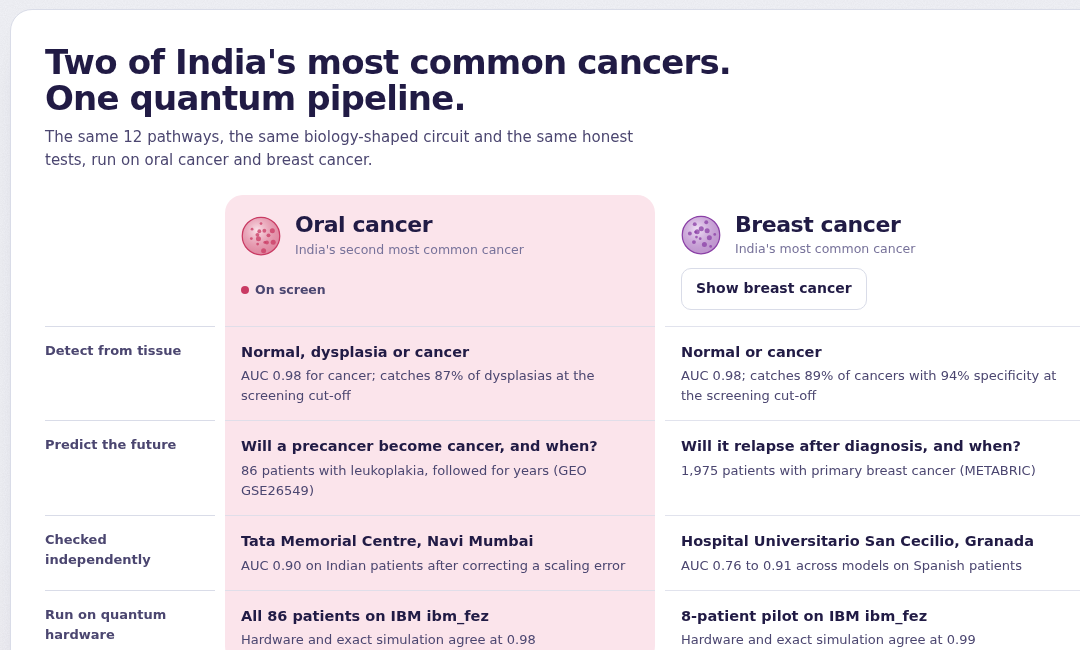
\includegraphics[width=0.78\textwidth]{app_two_cancers.png}
\caption{Two-cancer comparison on the web application's Overview page.}
\label{fig:app}
\end{figure}

% ------------------------------------------------------------------ 4
\section{Data}
All data are public. Each dataset is processed and standardised on its own; expression values are never pooled across datasets, and external cohorts are used once, after training (Table~\ref{tab:data}).

\begin{table}[H]
\centering
\caption{Cohorts used (2,573 samples).}
\label{tab:data}
\small
\begin{tabularx}{\textwidth}{@{}l Y l l@{}}
\toprule
\textbf{Cohort} & \textbf{Source} & \textbf{Samples} & \textbf{Use} \\
\midrule
Oral precancer & GEO GSE26549 \cite{saintigny} & 86 (35 progressed) & Progression (flagship) \\
Oral tissue & GEO GSE30784 \cite{chen}, Fred Hutchinson, USA & 229 (45 N, 17 D, 167 C) & Detection \\
Oral tissue, India & GEO GSE23558 \cite{ambatipudi}, Tata Memorial Centre & 32 (27 C, 5 N) & Independent check \\
Breast cancer & METABRIC \cite{curtis}, cBioPortal & 1,975 (800 relapses) & Relapse, subtype \\
Breast tissue & GEO GSE42568, Dublin City University & 121 (104 C, 17 N) & Detection \\
Breast tissue, Spain & GEO GSE10810, Hosp.\ Univ.\ San Cecilio & 58 (31 C, 27 N) & Independent check \\
Leukaemia & Golub et al.\ \cite{golub} & 72 & Calibration (AML vs ALL) \\
\bottomrule
\multicolumn{4}{@{}l}{\footnotesize N: normal, D: dysplasia, C: cancer.}
\end{tabularx}
\end{table}

% ------------------------------------------------------------------ 5
\section{Methodology}
\subsection{Pathway compression}
Single-sample gene set enrichment analysis (rank-normalised) \cite{barbie} scores each sample on 12 MSigDB Hallmark pathways \cite{liberzon}, fixed from cancer biology before any outcome was seen: MYC targets, E2F targets, G2/M checkpoint, mTORC1, unfolded protein response, oxidative phosphorylation, p53, DNA repair, hypoxia, epithelial--mesenchymal transition, TNF-$\alpha$ via NF-$\kappa$B, and inflammatory response. No feature is selected using outcomes.

\subsection{Quantum feature map}
Pathway $z$-scores become rotation angles $x_k = s\,\tfrac{\pi}{2}\tanh(z_k/2)$, with bandwidth $s$ chosen by cross-validation. Starting from Hadamard gates on 12 qubits, the circuit applies one or two Trotter steps of
\begin{equation}
H(\mathbf{x}) = \sum_{k} x_k Z_k + \sum_{(i,j)\in E} x_i x_j\, Z_i Z_j + \beta \sum_k X_k ,
\end{equation}
where $E$ is the \emph{pathway crosstalk graph}: two qubits interact only if their gene sets overlap (14 edges). Without seeing outcomes, it links the cell-cycle programmes (MYC, E2F, G2/M) and the inflammatory programmes (TNF-$\alpha$, inflammatory response, p53).

\subsection{Quantum kernels}
The projected quantum kernel \cite{huang2021} compares single-qubit Bloch vectors $\mathbf{r}_k$:
\begin{equation}
k(\mathbf{x},\mathbf{x}') = \exp\Big(-\gamma \sum_{k} \lVert \mathbf{r}_k(\mathbf{x}) - \mathbf{r}_k(\mathbf{x}') \rVert^2\Big).
\end{equation}
It needs only $X$, $Y$ and $Z$ expectations per qubit (three measurement settings per patient, so circuit count grows linearly with patients) and remains positive semi-definite under shot noise. The fidelity kernel \cite{havlicek} serves as the standard quantum comparator.

\subsection{Prediction models}
\begin{itemize}
\item \textbf{Detection:} support-vector machines on projected, fidelity and classical RBF kernels, compared with logistic regression, random forest and gradient boosting.
\item \textbf{Time-to-event:} a kernel-weighted Kaplan--Meier (Beran) estimator \cite{beran} over the 15 most similar patients gives a survival curve, a risk at the clinical horizon (3 years oral, 5 years breast), pathway attributions and the nearest cases; it abstains when too few similar patients exist.
\end{itemize}

\subsection{Quantum Readiness Check}
Before training, the geometric difference between quantum and classical kernels \cite{huang2021} bounds how much room quantum has on a dataset. Combined with a learning test and a held-out comparison on the real outcome, the check returns \emph{go}, \emph{wait} or \emph{classical}, and includes a positive control that must return \emph{go}. It runs in Python and in the browser.

% ------------------------------------------------------------------ 6
\section{Validation approach}
\begin{table}[H]
\centering
\caption{Validation controls.}
\begin{tabularx}{\textwidth}{@{}l Y@{}}
\toprule
\textbf{Control} & \textbf{Implementation} \\
\midrule
Plans before results & Analysis plans written before outcome analysis (OSF registration for prognosis; dated plans in the repository for detection). Later changes declared as dated amendments before they were run. \\
Equal budgets & Every model tunes hyperparameters by the same inner cross-validation; kernel bandwidths come from training folds only. \\
Resampling & Nested leave-one-out and repeated stratified cross-validation (5-fold $\times$ 10 repeats for detection; 20 $\times$ 5 for the oral cohort); bootstrap 95\% intervals. \\
Statistics & Projected quantum vs classical RBF as primary comparison; Wilcoxon signed-rank and Bouckaert--Frank corrected $t$-tests \cite{bouckaert}; Holm correction for secondary comparisons. \\
Controls & Engineered quantum-structured labels must produce a quantum win; the Readiness Check includes a control that must return \emph{go}. \\
External data & Independent cohorts used once, unchanged, after training; each dataset standardised on its own. \\
\bottomrule
\end{tabularx}
\end{table}

% ------------------------------------------------------------------ 7
\section{Results}
\subsection{Prognosis on real outcomes}
The quantum kernel matches classical methods on real outcomes but does not beat them (Table~\ref{tab:prog}, Figure~\ref{fig:prog}). On the oral cohort with nested leave-one-out, projected quantum scores 0.554, fidelity quantum 0.568 and classical RBF 0.580, with overlapping intervals. The projected kernel beats the standard fidelity kernel on the oral cohort ($p \approx 0.002$, Holm-corrected) while needing half the gates.

\begin{table}[H]
\centering
\caption{Quantum versus classical on real outcomes (C-index for survival, AUC for classification).}
\label{tab:prog}
\small
\begin{tabularx}{\textwidth}{@{}>{\raggedright\arraybackslash}p{3.1cm} l r c c Y >{\raggedright\arraybackslash}p{2.2cm}@{}}
\toprule
\textbf{Task} & \textbf{Data} & \textbf{$n$} & \textbf{Quantum} & \textbf{RBF} & \textbf{Best classical} & \textbf{Verdict} \\
\midrule
Oral cancer progression & GSE26549 & 86 & 0.601 & 0.613 & 0.643, elastic-net Cox & Parity \\
Breast cancer relapse & METABRIC & 1,975 & 0.582 & 0.582 & 0.662, NPI + pathways & Parity ($p=0.98$) \\
Breast subtype (basal) & METABRIC & 1,200 & 0.885 & 0.913 & 0.925, logistic & Classical ahead \\
Leukaemia (AML/ALL) & Golub & 72 & 0.857 & 0.903 & 0.941, logistic & Classical ahead \\
\bottomrule
\end{tabularx}
\end{table}

\begin{figure}[H]
\centering
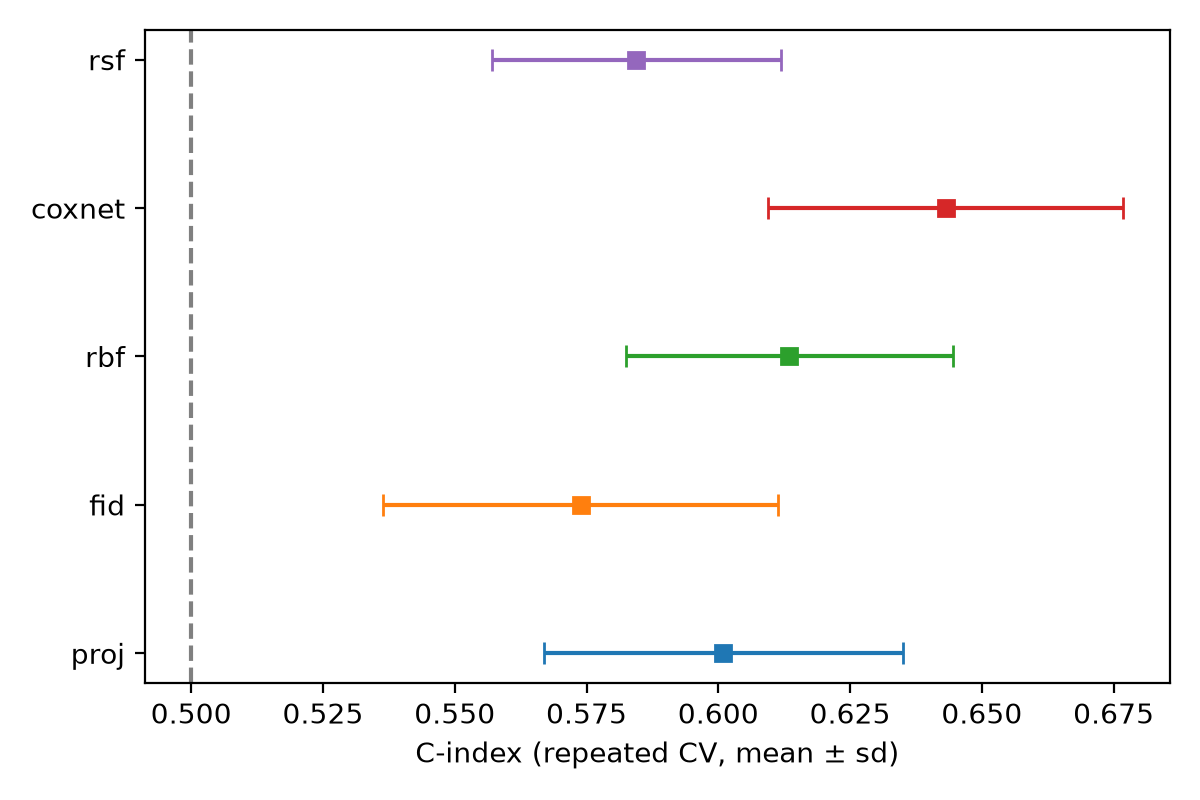
\includegraphics[width=0.49\textwidth]{cindex_forest.png}\hfill
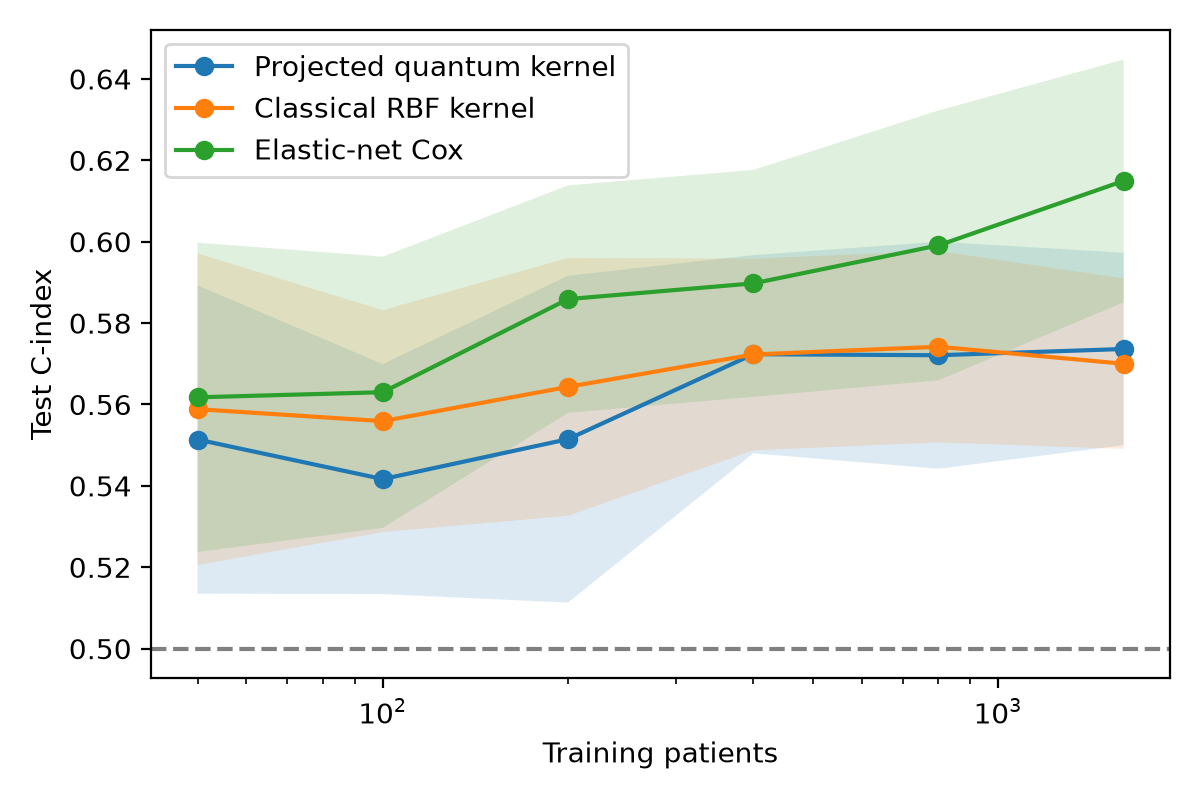
\includegraphics[width=0.49\textwidth]{metabric_size_curve.png}
\caption{Left: oral cohort C-index, 20 $\times$ 5 repeated cross-validation. Right: METABRIC test C-index as the training set grows from 50 to 1,600 patients.}
\label{fig:prog}
\end{figure}

\subsection{Detection from tissue}
Detection ranks well for every model, and quantum ties classical on every registered task (Table~\ref{tab:det}). For oral dysplasia, the default cut-off caught only 51\%; a declared screening cut-off (at least 90\% of positives on training folds, applied unchanged to held-out folds) raised this to 87\% while clearing 85\% of normal tissue. Cancer versus dysplasia (167 vs 17 samples) is not usable at default settings; with class weighting, an exploratory amendment, the kernel models reach AUC 0.87.

\begin{table}[H]
\centering
\caption{Detection from tissue, repeated cross-validation (5-fold $\times$ 10 repeats).}
\label{tab:det}
\small
\begin{tabularx}{\textwidth}{@{}Y l l l l Y@{}}
\toprule
\textbf{Task} & \textbf{Samples} & \textbf{Proj.\ quantum AUC} & \textbf{RBF AUC} & \textbf{Quantum vs RBF} & \textbf{Screening cut-off (sens./spec.)} \\
\midrule
Oral: cancer vs normal & 167 vs 45 & $0.980 \pm 0.026$ & 0.985 & $p=0.72$, tie & Default preferred: 97\% / 86\% \\
Oral: dysplasia vs normal & 17 vs 45 & $0.953 \pm 0.051$ & 0.957 & $p=0.83$, tie & 87\% / 85\%, NPV 95\% \\
Oral: cancer vs dysplasia & 167 vs 17 & $0.753 \pm 0.141$ & 0.813 & $p=0.22$, tie & 90\% / 49\% (not usable) \\
Breast: cancer vs normal & 104 vs 17 & $0.983 \pm 0.030$ & 0.948 & $p=0.45$, tie & 89\% / 94\% \\
\bottomrule
\end{tabularx}
\end{table}

\subsection{Independent checks}
Models trained on the main cohort were applied once to cohorts from other laboratories and platforms (Table~\ref{tab:ext}). The registered Indian check initially failed (projected quantum AUC 0.24). The cause was a scaling error rather than biology: gseapy rescales ssGSEA normalised enrichment scores across each whole dataset, so the two datasets' scores were on different scales. Re-run with each dataset standardised on its own, declared before it was run and labelled a post-hoc correction, the ranking transfers. In both cancers, cancer moves in the same direction in both datasets for 11 of 12 pathways. The default cut-off does not transfer: models catch nearly every cancer but clear only a minority of normal samples.

\begin{table}[H]
\centering
\caption{Independent checks, applied once (descriptive; bootstrap 95\% intervals).}
\label{tab:ext}
\small
\begin{tabularx}{\textwidth}{@{}Y l l r r@{}}
\toprule
\textbf{External cohort} & \textbf{Model} & \textbf{AUC (95\% CI)} & \textbf{Sensitivity} & \textbf{Specificity} \\
\midrule
\multirow{3}{=}{Oral: Tata Memorial Centre, India (27 C, 5 N)} & Projected quantum & 0.90 (0.78--0.99) & 93\% & 40\% \\
 & Classical RBF & 0.93 (0.82--1.00) & 93\% & 40\% \\
 & Logistic regression & 0.86 (0.66--1.00) & 93\% & 20\% \\
\midrule
\multirow{3}{=}{Breast: Granada, Spain (31 C, 27 N)} & Projected quantum & 0.79 (0.65--0.91) & 100\% & 41\% \\
 & Classical RBF & 0.87 (0.77--0.95) & 100\% & 41\% \\
 & Logistic regression & 0.91 (0.83--0.97) & 100\% & 33\% \\
\bottomrule
\end{tabularx}
\end{table}

\subsection{Where quantum helps, and why it ties here}
A positive control with labels engineered to carry quantum structure over real METABRIC features (geometric difference 6.75) \cite{huang2021} produces a clear quantum win: AUC 0.902 vs 0.614 with 25 training patients, 0.967 vs 0.731 with 50, and 0.999 vs 0.906 with 400 (Figure~\ref{fig:adv}). On the real outcome all models overlap. At the cross-validated bandwidth (0.25) each qubit's Bloch vector keeps almost its full length (mean 0.994, where 1 means no entanglement), so the quantum kernel behaves much like a classical one; at bandwidth 1 the vectors shorten to 0.685, so entanglement is available but the outcome does not reward it. The Readiness Check reaches the same verdict independently, consistent with the field's largest systematic review \cite{gupta}.

\begin{figure}[H]
\centering
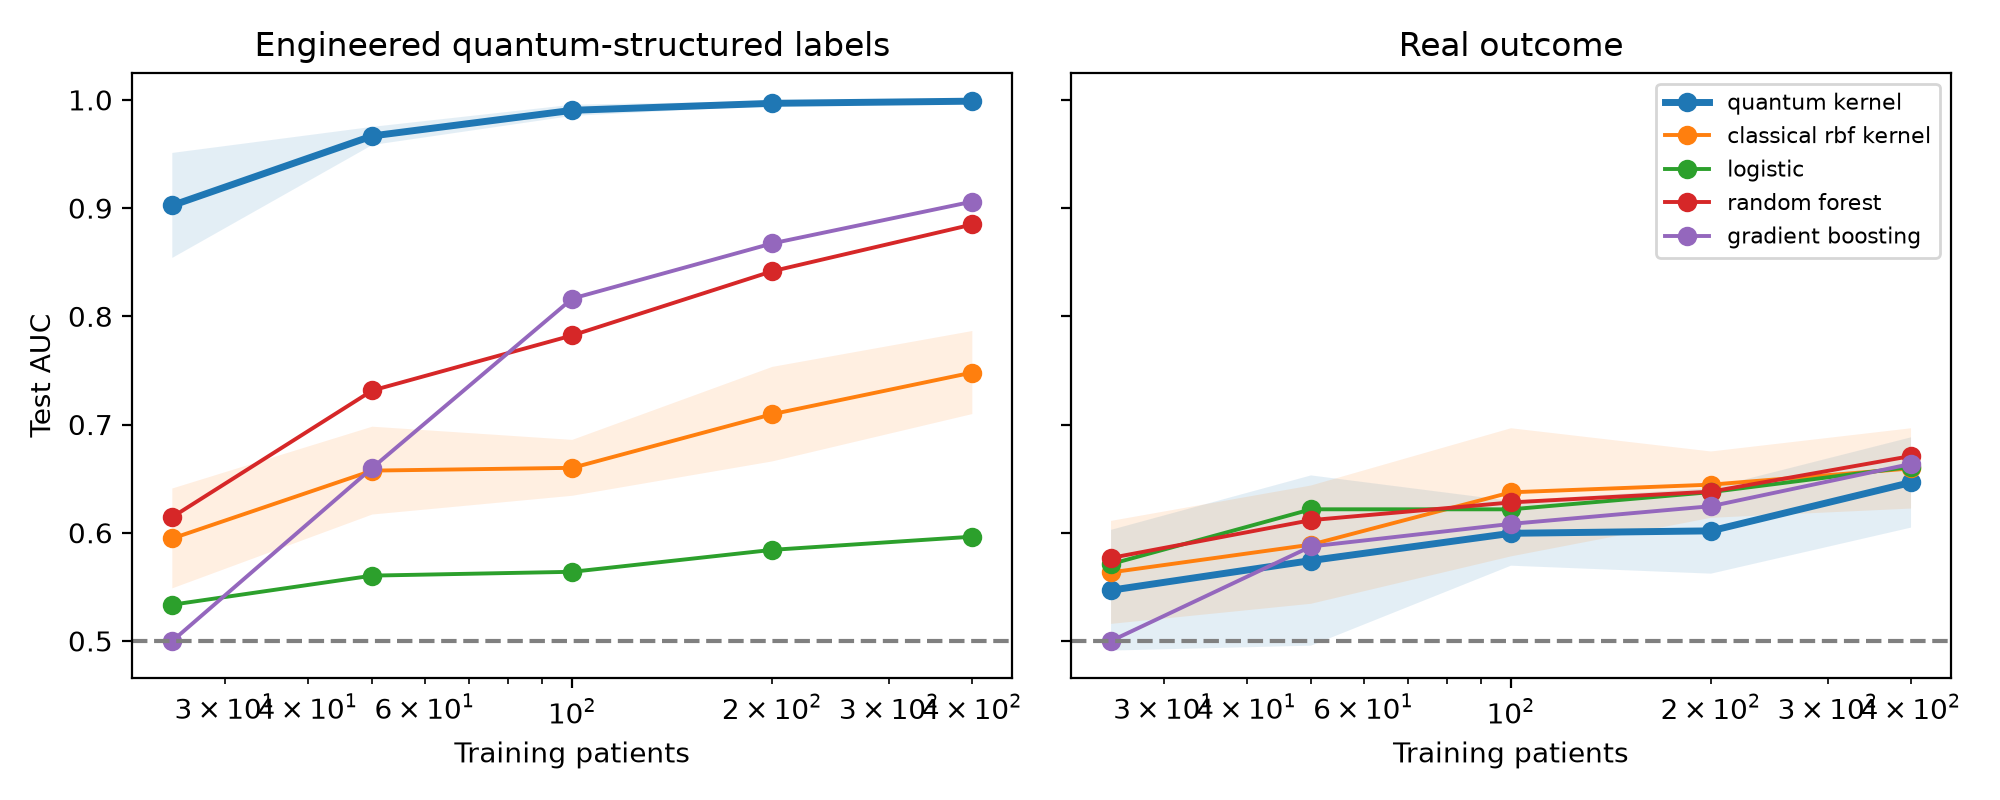
\includegraphics[width=\textwidth]{advantage_curve.png}
\caption{Test AUC against training patients. Left: engineered quantum-structured labels (synthetic by construction). Right: the real outcome.}
\label{fig:adv}
\end{figure}

\subsection{IBM quantum hardware}
The full oral cohort ran on IBM \texttt{ibm\_fez} (156-qubit Heron) through Qiskit Runtime (EstimatorV2, Batch mode, TREX readout mitigation), one circuit per patient measuring the 36 single-qubit expectations the projected kernel needs. The hardware kernel agrees with exact simulation at 0.979; the C-index gap (0.566 vs 0.593, same patients) is the cost of noise, not a separate accuracy claim. Three settings per patient gives 258 circuits for 86 patients instead of 3,655 pairwise circuits (14$\times$ fewer). In noisy simulation at 3\% two-qubit gate error, the gentle encodings lose at most 0.011 C-index on METABRIC.

\begin{table}[H]
\centering
\caption{Hardware runs and circuit cost on IBM Heron (Qiskit 2.5, optimisation level 3, best of 8 seeds, FakeFez calibration). Estimated fidelity is the product of calibrated gate and readout success rates.}
\label{tab:hw}
\small
\begin{tabularx}{\textwidth}{@{}Y l r r l@{}}
\toprule
\textbf{Circuit (12 qubits)} & \textbf{Kernel} & \textbf{2q gates} & \textbf{Depth} & \textbf{Fidelity / agreement} \\
\midrule
SANKET, 1 step, \texttt{ibm\_fez}: oral, 86 patients & Projected & 49 & 19 & Kernel agreement 0.979 \\
SANKET, 1 step, \texttt{ibm\_fez}: METABRIC, 8 patients & Projected & 49 & 19 & Bloch correlation 0.991 \\
SANKET pathway topology, 2 steps & Projected & 94 & 33 & 0.67 (estimated) \\
SANKET pathway topology, 2 steps & Fidelity & 188 & 70 & 0.48 (estimated) \\
All-to-all Hamiltonian, 2 steps & Projected & 433 & 151 & 0.21 (estimated) \\
Standard ZZ feature map (full), 2 reps & Fidelity & 906 & 333 & 0.04 (estimated) \\
\bottomrule
\multicolumn{5}{@{}l}{\footnotesize IBM job identifiers: oral \texttt{davbc6il7guc73cekc8g}; METABRIC \texttt{davjuitj371s73dn2570}.}
\end{tabularx}
\end{table}

\begin{figure}[H]
\centering
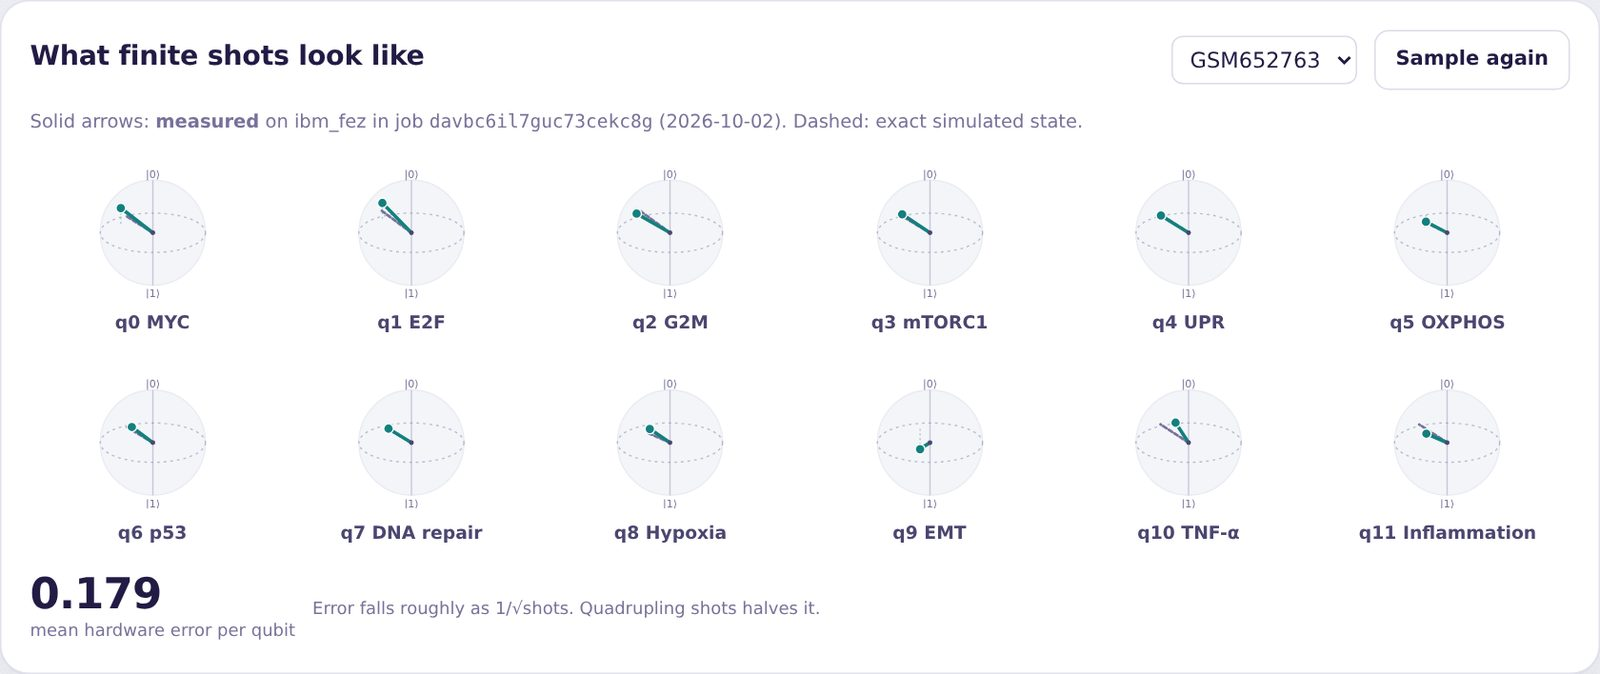
\includegraphics[width=0.8\textwidth]{hardware-measured.jpg}
\caption{One patient's 12 qubits measured on \texttt{ibm\_fez} (solid) against the exact simulated state (dashed).}
\end{figure}

\subsection{Clinical usefulness}
On the oral cohort at three years, with a referral rule set to catch at least 90\% of progressions, the projected quantum kernel refers 84\% of patients against 90\% for the classical RBF kernel, with a higher negative predictive value (86\% vs 76\%); elastic-net Cox does better still (78\% referred, NPV 89\%). On METABRIC, adding the 12 pathways to the clinical Nottingham Prognostic Index raises the C-index from 0.639 to 0.662. Across METABRIC's five recruitment cohorts, the quantum kernel scores 0.595 against 0.587 for the classical kernel.

% ------------------------------------------------------------------ 8
\section{Limitations and risks}
\begin{table}[H]
\centering
\caption{Known limitations, impact and planned response.}
\small
\begin{tabularx}{\textwidth}{@{}Y Y Y@{}}
\toprule
\textbf{Limitation} & \textbf{Impact} & \textbf{Response} \\
\midrule
No quantum advantage on real outcomes & Quantum value rests on cost, design and readiness, not accuracy & Reported as found; Readiness Check advises when to stay classical \\
Small cohorts: 86 progression patients; 17 dysplasias & Wide intervals; cancer vs dysplasia exploratory & More data through a clinical partner \\
Few external normals (5 India, 27 Spain) & Specificities fragile & Indian training data for calibration \\
Indian correction is post hoc & Weaker evidence than a registered result & Declared and labelled; original result retained \\
Cut-offs do not transfer across platforms & Local calibration required before any use & Calibrate per site and platform \\
Modest prognostic accuracy (C-index 0.62--0.66) & Not clinically ready & Positioned as research and decision support \\
Cost of gene-expression input & Barrier to routine use in India & Evaluate a small targeted gene panel \\
Hardware covers 86 + 8 patients; fidelities estimated & Limited hardware evidence & Further runs as access allows \\
\bottomrule
\end{tabularx}
\end{table}

SANKET is a research prototype and decision support for clinicians. It is not a medical device and must not be used for diagnosis or treatment decisions.

% ------------------------------------------------------------------ 9
\section{Next steps}
\begin{table}[H]
\centering
\caption{Roadmap.}
\begin{tabularx}{\textwidth}{@{}Y l@{}}
\toprule
\textbf{Item} & \textbf{Status} \\
\midrule
Engine, detection and prognosis on two cancers, IBM hardware run, web prototype & Complete \\
Declared amendments: dysplasia screening cut-off, Indian check correction, class weighting & Complete \\
Breast cancer detection with an independent check & Complete \\
Public deployment of the web application; demonstration video & In progress \\
Indian training data for oral and breast cancer through a clinical partner & Planned \\
Ethics-approved (IEC) pilot with an oral oncology unit on de-identified data, under the DPDP Act, 2023 & Planned \\
Small targeted gene panel to lower input cost & Planned \\
Port to Indian quantum hardware under the National Quantum Mission & Planned \\
\bottomrule
\end{tabularx}
\end{table}

% ------------------------------------------------------------------ appendices
\appendix
\section{Reproducibility}
Every number in this report is produced by the repository from public data; result files are committed under \texttt{out/}.

\begin{table}[H]
\centering
\small
\begin{tabularx}{\textwidth}{@{}l Y@{}}
\toprule
\textbf{Purpose} & \textbf{Command} \\
\midrule
Registered benchmarks & \texttt{python -m engine.classify --task <task>} \\
Oral declared amendments & \texttt{python -m engine.oral\_amendments --a1 --a2 --a3} \\
Breast detection & \texttt{python -m engine.breast\_detect --screening --external} \\
Readiness Check & \texttt{python -m engine.readiness} \\
Web application bundles & \texttt{python -m engine.export\_detect}; \texttt{python -m engine.export\_app\_cohorts} \\
\bottomrule
\end{tabularx}
\end{table}

\begin{thebibliography}{99}\small
\bibitem{havlicek} V.~Havl\'{i}\v{c}ek \emph{et al.}, ``Supervised learning with quantum-enhanced feature spaces,'' \emph{Nature} 567, 209--212 (2019).
\bibitem{huang2021} H.-Y.~Huang \emph{et al.}, ``Power of data in quantum machine learning,'' \emph{Nat.\ Commun.} 12, 2631 (2021).
\bibitem{huang2022} H.-Y.~Huang \emph{et al.}, ``Quantum advantage in learning from experiments,'' \emph{Science} 376, 1182--1186 (2022).
\bibitem{gupta} R.~S.~Gupta \emph{et al.}, ``A systematic review of quantum machine learning for digital health,'' \emph{npj Digit.\ Med.} 8, 237 (2025).
\bibitem{bowles} J.~Bowles, S.~Ahmed and M.~Schuld, ``Better than classical? The subtle art of benchmarking quantum machine learning models,'' arXiv:2403.07059 (2024).
\bibitem{qiskit} A.~Javadi-Abhari \emph{et al.}, ``Quantum computing with Qiskit,'' arXiv:2405.08810 (2024).
\bibitem{saintigny} P.~Saintigny \emph{et al.}, ``Gene expression profiling predicts the development of oral cancer,'' \emph{Cancer Prev.\ Res.} 4, 218--229 (2011).
\bibitem{curtis} C.~Curtis \emph{et al.}, ``The genomic and transcriptomic architecture of 2,000 breast tumours,'' \emph{Nature} 486, 346--352 (2012).
\bibitem{golub} T.~R.~Golub \emph{et al.}, ``Molecular classification of cancer: class discovery and class prediction by gene expression monitoring,'' \emph{Science} 286, 531--537 (1999).
\bibitem{liberzon} A.~Liberzon \emph{et al.}, ``The Molecular Signatures Database Hallmark gene set collection,'' \emph{Cell Syst.} 1, 417--425 (2015).
\bibitem{barbie} D.~A.~Barbie \emph{et al.}, ``Systematic RNA interference reveals that oncogenic KRAS-driven cancers require TBK1,'' \emph{Nature} 462, 108--112 (2009).
\bibitem{beran} R.~Beran, ``Nonparametric regression with randomly censored survival data,'' Technical report, University of California, Berkeley (1981).
\bibitem{bouckaert} R.~R.~Bouckaert and E.~Frank, ``Evaluating the replicability of significance tests for comparing learning algorithms,'' \emph{PAKDD}, 3--12 (2004).
\bibitem{chen} C.~Chen \emph{et al.}, ``Gene expression profiling identifies genes predictive of oral squamous cell carcinoma,'' \emph{Cancer Epidemiol.\ Biomarkers Prev.} 17, 2152--2162 (2008).
\bibitem{ambatipudi} S.~Ambatipudi \emph{et al.}, ``Genomic profiling of advanced-stage oral cancers reveals chromosome 11q alterations as markers of poor clinical outcome,'' \emph{PLoS One} 7, e32436 (2012).
\end{thebibliography}

\end{document}